\documentclass[dvipdfmx,autodetect-engine]{article}
%---------------------package
\usepackage{geometry}
\usepackage{amssymb}
\usepackage{amsmath}
\usepackage{amsthm}
\usepackage{tikz}
\usetikzlibrary{positioning}
%----------------------------命令定義
\DeclareMathOperator{\Hom}{Hom}
\DeclareMathOperator{\End}{End}
\DeclareMathOperator{\GL}{GL}
\DeclareMathOperator{\gl}{gl}
\DeclareMathOperator{\sllie}{sl}
\DeclareMathOperator{\sublie}{\mathfrak{a}}
\DeclareMathOperator{\lie}{\mathfrak{g}}
\DeclareMathOperator{\cartan}{\mathfrak{h}}
\DeclareMathOperator{\U}{U}


%---------------------------make title
\title{量子群の表現論}
\author{}
\date{}
%-----------------------------document
\begin{document}
\maketitle
\section{はじめに}
\label{sec_intro}
      量子群,特に$A_{r-1}^{(1)}$型量子群を中心にまとめます.詳しい証明は多分省きますが,方針を書いておくつもりです.なるべく理論の全体像がわかるように書きます.単なるFact集.セミナー用ノート.文献は,ArikiさんのRepresetation over Quantum Algebras of type $A_{r-1}^{(1)}$がメイン.
\section{包絡環とPBW定理}
\label{sec_enveloping_algebras}
\subsection{リー環}
    量子群はリー環の包絡環を変形することで得られます.ここではリー環の定義から始めて,包絡環の基本的なことを書きます.目標はPBW定理です.
    \begin{}
      \label{def_lie}
      $\mathbb{C}$上のベクトル空間$\lie$にblacketなどと呼ばれる双線型写像$[\cdot, \cdot]:\lie \otimes \lie \to \lie$が与えられていて,これが
      \begin{enumerate}
          \item \label{def_lie_antisym} $[x, y] = - [y, x] \quad (\forall x, y \in \lie)$,
          \item \label{def_lie_jacobi} $[x, [y, z]] + [y, [z, x]] + [z, [x, y]] = 0 \quad (\forall x,y,z \in \lie)$,
      \end{enumerate}
      を満たすとき,$\lie$を\textbf{リー環}という.(\ref{def_lie_jacobi})はJacobi identityという.また(\ref{def_lie_antisym})は$[x,x] = 0\,(\forall x \in \lie)$と同値.
      \qed
    \end{def}

    これは非結合的環とでも言うべきもの.重要な例は$\End(V)$.
    \begin{example}
    \label{ex_gl}
        $\End(V)$は
        \[
          [X, Y] = XY - YX
        \]
        でリー環になる.
        $\End(V)$をこのリー積でリー環とみなすとき,$\gl(V)$と書いたりする.
        これは一般線型リー環,general linear lie algbra などと呼ばれる.
        \qed
    \end{example}

    一般に結合環には上のリー積で,リー環の構造が入ります.

    ここから少し基本的な定義が続きます.
    \begin{definition}
    \label{def_sublie_ideal}
        部分空間$\sublie \subset \lie$が
        \[
           [\sublie, \sublie] \subset \sublie
        \]
        を満たす時,$\sublie$を$\lie$の\textbf{部分リー環}という.
        特に,$[\sublie, \sublie] = 0$なら可換部分リー環という.
        また,
        \[
           [\lie, \sublie] \subset \sublie
        \]
        を満たす時は$\lie$の\textbf{イデアル}であるという.
        \qed
    \end{definition}

    \begin{definition}
    \label{def_hom}
      リー環$\lie$, $\mathfrak{h}$に対し,
      $\mathbb{C}$線形写像$\rho: \lie \to \mathfrak{h}$が
      \[
          \rho([x, y]) = [\rho(x), \rho(y)]
      \]
      を満たす時,$\rho$をリー環の準同型という.
      また,準同型$\rho: \lie \to \gl(V)$と$V$の組$(\rho, V)$を$\lie$の\textbf{表現}という.
      \qed
    \end{definition}
    
    表現あればそこから$V$に$\lie$の作用が定まり$V$は$\lie$-加群になります,逆に$\lie$-加群$V$があればそこから表現を定めることができます.
    また$\gl(V)$にはExample \ref{ex_gl}のリー積が入っているので,
    \[
        \rho([x, y]) = [\rho(x), \rho(y)] = \rho(x)\rho(y) - \rho(y)\rho(x)
    \]
    です.

\subsection{包絡環}
    次にリー環の包絡環を定義します.リー環は非結合的な環でしたが,その包絡環を考えることで結合環の話にできます.さらにこれはPBW基底といういい基底を持ちます.以下単に環といったら$\mathbb{C}$上の単位的結合環を考えることにします.

    \begin{definition}
    \label{def_env}
        リー環$\lie$.結合環$A$と準同型$f:\lie \to A$の組$(A, f)$の中で次の意味でuniversalなものを$L$の\textbf{包絡環}という.
        \begin{itemize}
          \item 別の組$(B, g)$がある時,結合代数の準同型$h: A \to B$であって,$g = h \circ f$を満たすものが一意的に存在する.
        \end{itemize}
        \[
            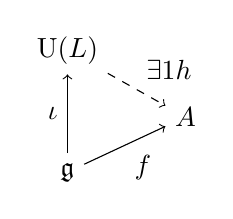
\begin{tikzpicture}
                \node (L) {$\lie$};
                \node[above =of L] (UL) {$\U(L)$};
                \node (A) at (1.5,0.7) {$A$};
                \draw[->] (L) --node[left] {$\iota$} (UL);
                \draw[->] (L) --node[below right] {$f$} (A);
                \draw[dashed,->] (UL) --node[above right] {$\exists1 h$} (A);
            \end{tikzpicture}
        \]

        リー環$\lie$の包絡環を$(\U(L), \iota)$とかく.
        \qed
    \end{definition}

    包絡環に関して次が成立します.
    \begin{proposition}
        包絡環は同型を除いてただ一つ存在する.
        \qed
    \end{proposition}
    次の手順で示します.
    
    \begin{lemma}
        \begin{itemize}
          \item 包絡環は存在すればただ一つ.
          \item 環$U$
        \end{itemize}
    \end{lemma}
  \end{document}
